 \section{Defined Class Description ODP}\begin{description}
\item [CLASSIFICATION:] Good Practice.

\item [MOTIVATION:] If-Then structures are very common and intuitive and this ODP offers the possibility of representing them within OWL DL expressivity.

\item [AIM:] To simulate an If-Then of the type: if something fullfills certain conditions, it should have a further given attribute.

\item [STRUCTURE:] See Figure \ref{odp:DefinedClass_Description_abstract}.
\begin{figure}[]\centering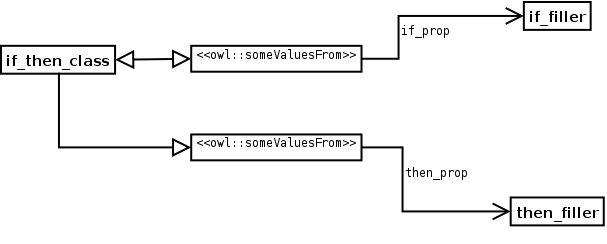
\includegraphics[width=\textwidth]{Catalogue/DefinedClass_Description_abstract}\caption{\label{odp:DefinedClass_Description_abstract} Abstract structure of the Defined Class Description ODP.}\end{figure}

\item [SAMPLE:] See Figure \ref{odp:DefinedClass_Description_instance}.
\begin{figure}[]\centering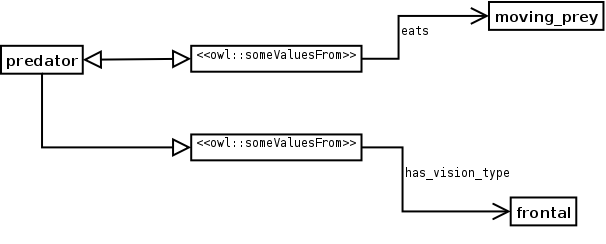
\includegraphics[width=\textwidth]{Catalogue/DefinedClass_Description_instance}\caption{\label{odp:DefinedClass_Description_instance} Sample structure of the Defined Class Description ODP.}\end{figure}

\item [ELEMENTS:] the important elements are the class that is being used to simulate the rule and the properties that are used in the condition (the equivalent restrictions) and the conclusion (the neccesary restrictions).

\item [RESULT:] The If-Then rule is represented in the ontology and can be used, for example, when adding new classes and performing reasoning: if a class fulfill the If condition, it will have also the Then attribute.

\item [REFERENCES: ] ~\begin{itemize}
\item Alan Rector, Nick Drummond, Matthew Horridge, Jeremy Rogers, Holger Knublauch,  Robert Stevens, Hai Wang, Chris Wroe. OWL Pizzas: Practical Experience of Teaching OWL-DL: Common Errors and Common Patterns. In Proceedings of  the European Conference on Knowledge Acquistion, 2004. LNCS- LNAI 3257, Springer-Verlag.pp 63-81.\end{itemize}
\item [URL: ] \url{http://www.gong.manchester.ac.uk/odp/owl/Good_Practice_ODP/DefinedClass_Description.owl} \end{description}